\documentclass[a4paper, 11pt]{article}

\usepackage[utf8]{inputenc}
\usepackage[T1]{fontenc}
\usepackage[french]{babel}
\usepackage{lscape}
\usepackage{lmodern}
\usepackage{enumitem}
\usepackage{amsmath}
\usepackage{amssymb}
\usepackage{mathrsfs}
\usepackage[load-configurations = abbreviations, separate-uncertainty=true]{siunitx}
\usepackage{graphicx}
\usepackage{epstopdf}
\usepackage[]{subcaption}
\usepackage{bm}
\usepackage[]{animate}
\usepackage[justification=centering]{caption}
\usepackage{wrapfig}
\usepackage{multirow}
\usepackage{multicol}
\usepackage[multiple]{footmisc}
\usepackage[hidelinks]{hyperref}
\usepackage{eurosym}
\usepackage{url}
\usepackage[top=2cm, bottom=2cm, left=2cm, right=2cm]{geometry}
\usepackage{pdfpages}
\usepackage{fancyhdr}
\usepackage{listings}
\usepackage{tikz}
\usepackage{tikz-3dplot}
\usetikzlibrary{shapes, decorations.pathmorphing, decorations.markings, arrows}

\pagestyle{fancy}
\date{\today}

\graphicspath{{./fig/}}
\epstopdfsetup{outdir=./fig/}

\renewcommand{\headrulewidth}{0.4pt}
\fancyhead[C]{} 
\fancyhead[L]{Rapport semestriel}
\fancyhead[R]{26 avril 2021}

\renewcommand{\footrulewidth}{0.4pt}
\fancyfoot[C]{\textbf{page \thepage}} 
\fancyfoot[L]{Projet DS3DLive}
\fancyfoot[R]{Maxime \textsc{Teil}}

\renewcommand{\tablename}{\textsc{Tableau}}

\lstset{language=Python, basicstyle=\ttfamily, numbers=left, breaklines=true, showspaces=false, showstringspaces=false}

\begin{document}

% Title page
\thispagestyle{plain}
\begin{center}
	\fbox{\Large{Rapport semestriel}}
	\vspace{2em}\\
	{\Large Projet DS3DLive} \vspace{2em}\\
	\begin{tabular}{c}
		\hline
		26 avril 2021 \vspace{.8em} \\
		Maxime \textsc{Teil} (LGP2 - Grenoble INP)\\
		\href{mailto:maxime.teil@lgp2.grenoble-inp.fr}{maxime.teil@lgp2.grenoble-inp.fr}\\
		04~76~82~69~43\\
		\hline
	\end{tabular} \vspace{2em}\\
	\begin{tikzpicture}[scale=1.]
		\draw (-2em, 0) node[left]{\includegraphics[height=3.5em]{../../lgp2.png}} ;
		\draw (2em, 0) node[right]{\includegraphics[height=4em]{../../Grenoble_INP.png}} ;
	\end{tikzpicture} \vspace{2em}
	\paragraph{Partenaires\\}
		~\\\vspace{1em}
		\begin{tikzpicture}[scale=1.]
			\draw (0, 0) node[]{\includegraphics[height=3.3em]{../../reactivip.png}} ;
			\draw (12em, 0) node[]{\includegraphics[height=4em]{../../ahlstrom.png}} ;
			\draw (22em, 0) node[]{\includegraphics[height=4.5em]{../../gerex.jpg}} ;
			\draw (32em, 0) node[]{\includegraphics[height=4em]{../../cmtc.png}} ;
		\end{tikzpicture} \vspace{2em}
	\paragraph{Projet financé par la région Auvergne-Rhône-Alpes\\}
		~\\\vspace{1em}
		\begin{tikzpicture}[scale=1.]
			\draw (0, 0) node[]{\includegraphics[height=3.5em]{../../region.png}} ;
		\end{tikzpicture} \vspace{2em}
\end{center}

\newpage\null
\newpage
\tableofcontents

% Rapport
\newpage
Ce rapport semestriel est le premier depuis le lancement du projet DS3DLive le 1$^\text{er}$ novembre 2020. Il a pour vocation de faire un rappel sur les objectifs qui ont été fixés lors de la réunion de lancement avec l'ensemble des partenaires, d'informer sur l'état d'avancement depuis cette date, de détailler l'ensemble des tâches accomplies et de faire un point sur la gestion actuelle du projet.
\\Une première partie se contentera de rappeler le planning envisagé lors du lancement et en fera une comparaison avec le planning réel. Il sera ensuite fait une prévision sur le planning des mois qui viennent.
\\Une présentation du montage d'essais en statique sera ensuite menée. Ce montage à pour objectif de répondre à l'ensemble des problématiques liées à la caractérisation par une technique de stéréovision en statique.
\\Le dispositif étant constitué de capteurs numériques, il est alors nécessaire de générer des codes de programmation pour mettre en \oe{}uvre les routines liées au projet. Pour cela, une librairie développée en Python a été crée et sera présentée.
\\Enfin, quelques points de discussion concernant la gestion du projet seront proposés.
	
	
\section{\'Etat d'avancement}
	Un rappel est fait ici concernant l'organisation du travail dans ce projet. Quatre tâches principales ont été déterminées :
	\begin{description}
		\item[WP1 :] Mise en place et développement technologique du dispositif d’imagerie par stéréovision ;
		\item[WP2 :] Développement de routines d’analyse d’images et de stéréocorrélation ;
		\item[WP3 :] Applications en statique ;
		\item[WP4 :] Applications en dynamique sur pilote de laboratoire ou machine semi-industrielle.
	\end{description}
	\begin{figure}[b]\centering
		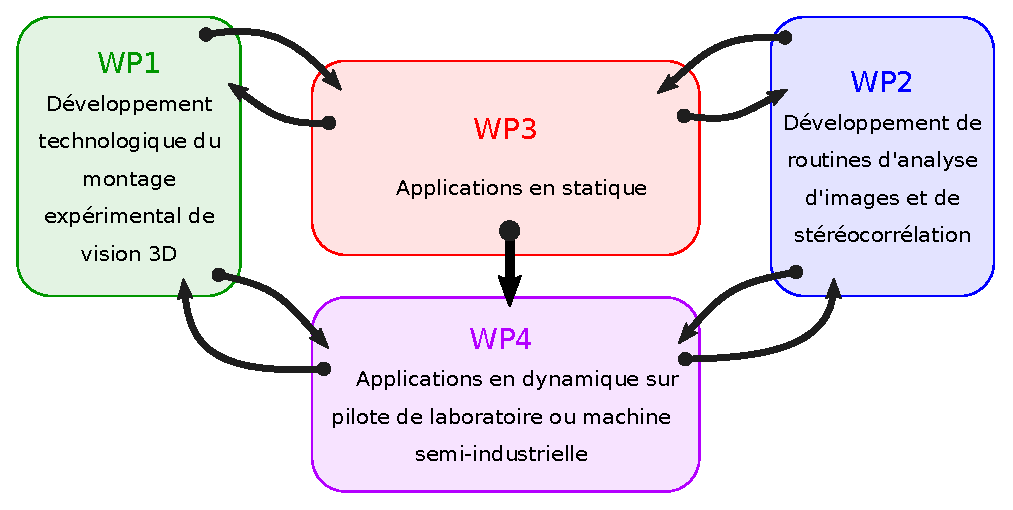
\includegraphics[width=.6\linewidth]{taches.eps}
		\caption{\label{fig:taches}Organisation du projet sous forme de tâches principales}
	\end{figure}
	La figure \ref{fig:taches} met en avant les interactions entre ces différentes tâches. WP1 et WP2 sont les tâches prioritaires car elles sont toutes deux nécessaire à la réalisation des autres tâches. WP3 doit être réalisée avant WP4 afin d'assurer une réponse aux problématiques de manière progressive, et donc certainement plus efficace.
	\paragraph{Planning prévisionnel du début de projet et planning réel\\}
	Un planning prévisionnel a été présenté en début de projet lors de la réunion de lancement. Le diagramme associé est présenté sur la figure \ref{fig:gantt_previsionnel}. Sur ce dernier est mis en avant la date actuelle grâce à la présence d'une ligne verticale pointillée. \`A ce jour, une grande partie du travail de mise en place du dispositif est censé être réalisé et le travail numérique doit être bien entamé. Des premiers essais en statique doivent avoir été menés afin de faire progresser le développement expérimental et numérique (WP1 et WP2).
	\begin{figure}\centering
		\begin{tikzpicture}
			\draw (0, 0) node {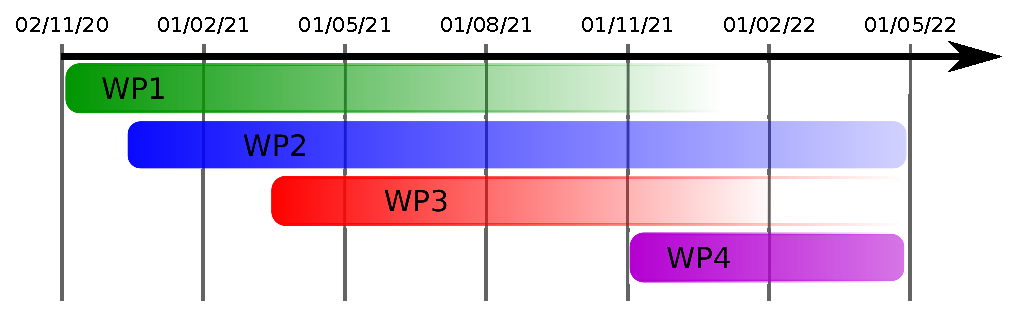
\includegraphics[width=.8\linewidth]{gant.eps}};
			\draw[densely dashed, line width=.2em] (-6em, -5.5em) -- ++(0, 10em);
		\end{tikzpicture}
		\caption{\label{fig:gantt_previsionnel}Planning prévisionnel}
	\end{figure}
	\\Qu'en est-il du planning réellement réalisé jusqu'à aujourd'hui ?
	\\Le diagramme peut rester tel quel à la condition que la tâche WP2 soit légèrement modifiée, ce qui précise encore plus l'organisation du travail.
	\begin{description}
		\item[WP2 :] Développement de routines \emph{de calibration des systèmes optiques,} d’analyse d’images et de stéréocorrélation.
	\end{description}
	En effet, il est primordial d'étalonner le système optique avant de procéder au traitement des images, et cela fait partie du travail numérique. Modification faite, le planning prévisionnel est respecté. Les prochains paragraphes ont pour objectif de présenter dans les détails les avancées concernant les tâches WP1, WP2 et WP3. De manière plus globale, le montage est opérationnel et peut être monté sur la machine pilote à tout moment : WP1 est donc très bien avancé. Une librairie Python permet de calibrer les caméras et d'étalonner le système de stéréovision afin de permettre certaine mesures de position dans l'espace : WP2 s'est donc bien déroulé jusqu'à présent. Enfin, des premiers essais de caractérisation 3D ont été menés afin de s'assurer de la fonctionnalité du dispositif expérimental et de la calibration du système : les caractérisations en statique sont donc possibles malgré certains efforts d'optimisation à fournir pour la suite.

\section{Montage du dispositif en statique}
	L'objectif du projet est d'être en capacité de monter un dispositif de caractérisation par stéréovision sur une une machine de production. Une première étape consiste à ne traiter que des caractérisations hors production, c'est-à-dire sur des papiers qui sont statiques. Cela permet, dans un premier temps, de ne se focaliser que sur les aspects liés au montage et à l'architecture algorithmique du projet. Lorsque l'ensemble des ces tâches primordiales seront correctement traitées, il sera nécessaire de considérer l'aspect dynamique pour permettre de rendre le dispositif fonctionnel à l'échelle de la production semi-industrielle. Le dispositif présenté dans cette partie est la version adaptée au cas d'études en statique. Il est envisagé d'y apporter certaines corrections ou modifications dans sa version d'études en dynamique, notamment en ce qui concerne le système optique.
	\subsection{Système optique}
		Puisque dans cette partie le sujet ne bouge pas, il n'est pas nécessaire de considérer une caméra haute-performance capable de délivrer un flux important d'images à traitée. Il est cependant nécessaire de considérer des capteurs d'images dont la définition est celle attendue dans ce projet. Afin de ne pas générer trop de transformations liées à la distorsion lors de la prise de vue, il est choisi d'utiliser des objectifs de type appareil photographique numérique (APN) réflex dont la distance focale ne soit pas inférieure à \SI{24}{\milli\meter}. Pour ces raisons il a été fait le choix d'un ensemble de deux APN réflex de la marque Canon et du modèle EOS 1200D et de deux objectifs de la marque Canon et du modèle EF-S \SI{24}{\milli\meter} f/\num{2.8} STM dont les caractéristiques sont données, respectivement, dans les figures \ref{fig:caracteristiques_APN} et \ref{fig:caracteristiques_objectif}.
		\begin{figure}\centering
			\begin{subtable}[b]{.5\linewidth}
				\begin{tabular}{>{\bfseries}r@{\hspace{1em}}l}
					\hline
					Format & APS-C (\SI{22.3 x 14.9}{\milli\meter})\\
					Pixels effectifs & \num{18}~MPx \\
					Ratio de format & 3: 2 \\
					Filtre passe bas & intégré\\
					\hline\vspace{.5em}
				\end{tabular}
				\caption{}
			\end{subtable}
			\begin{subfigure}[b]{.45\linewidth}
				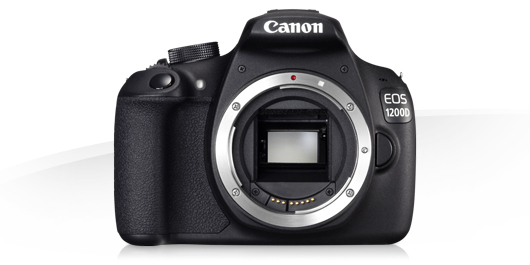
\includegraphics[width=\linewidth]{canonEOS1200D.jpg}
				\caption{}
			\end{subfigure}
			\caption{\label{fig:caracteristiques_APN}(a) Caractéristiques du capteur de l'APN EOS 1200D de chez Canon et (b) photographie de l'appareil. Source : \href{https://www.canon.fr/for_home/product_finder/cameras/digital_slr/eos_1200d/specification.html}{www.canon.fr}.}
		\end{figure}
		\begin{figure}\centering
			\begin{subtable}[b]{.5\linewidth}
				\begin{tabular}{>{\bfseries}r@{\hspace{1em}}l}
					\hline
					Focale équivalente (\SI{36 x 24}{\milli\meter}) & \SI{38}{\milli\meter}\\
					Distance minimale mise au point & \SI{160}{\milli\meter}\\
					Autofocus motorisé & oui\\
					Angle de champ horizontal & \ang{59;10;}\\
					Angle de champ vertical & \ang{50;35;}\\
					\hline\vspace{.05em}
				\end{tabular}
				\caption{}
			\end{subtable}
			\begin{subfigure}[b]{.45\linewidth}
				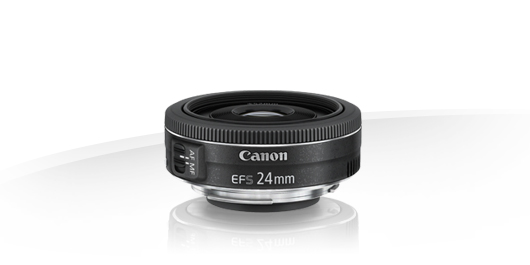
\includegraphics[width=\linewidth]{canonEFS24mm.jpg}
				\caption{}
			\end{subfigure}
			\caption{\label{fig:caracteristiques_objectif}(a) Caractéristiques de l'objectif EF-S \SI{24}{\milli\meter} f/\num{2.8} STM de chez Canon et (b) photographie de l'objectif. Source : \href{https://www.canon.fr/lenses/ef-s-24mm-f-2-8-stm-lens/specification.html}{www.canon.fr}.}
		\end{figure}
		\\Le capteur ainsi choisi permet d'obtenir une taille de pixel de l'ordre de \SI{70}{\micro\meter} en considérant un champ horizontal de approximativement \SI{35}{\centi\meter}. D'après le résultat présenté au paragraphe \ref{section:Alicona}, cette résolution permettrait de définir un pli par l'intermédiaire d'une dizaine de pixels.
		\\Afin de garantir une relativement bonne répétabilité lors des essais, chaque APN est associé à un objectif et l'ensemble est étiqueté "gauche" ou "droit". Les erreurs expérimentales liées aux capteurs et objectifs sont donc répétées pour chaque prise de mesures sur les images. D'un point de vue pratique, la calibration est faite pour chaque couple APN-objectif, ce qui permet d'obtenir des matrices de calibration et coefficients de distorsion qui sont propres à chacun de ses couples. Si les appareils ou les objectifs ne sont pas échangés alors ces propriétés peuvent être sauvegardées puis rechargées.
		\\L'enregistrement des images se fait au format JPEG haute qualité (\num{18}~MPx) sur carte SD insérée dans l'APN. Les traitements et post-traitements sont réalisés après la séance de prises de vue. L'ensemble des campagnes de prises de vue sont donc détaillées dans le cahier de laboratoire. Il est fait mention de la date, l'heure, le sujet de la prise de vue et les liaisons entre sujets et noms des images.
	
	\subsection{Assemblage structurel et fonctionnel}
		Les systèmes optiques sont censés pouvoir se fixer de manière permanente ou temporaire sur une coucheuse semi-industrielle. Dans le cadre de ce projet, et dans un premier temps, le choix se porte sur la machine pilote présente au laboratoire LGP2. Une structure a donc été imaginée afin de pouvoir fixer les systèmes optiques sur cette machine, tout en gardant la possibilité de régler le système de stéréovision. L'assemblage est présenté sur la figure \ref{fig:dispositif_statique} : il est constitué de poutres métalliques de section circulaire creuse de \SI{30}{\milli\meter} de diamètre extérieur. Différentes liaisons sont présentes afin de permettre les réglages suivants :
		\begin{itemize}
			\item Distance entre les deux caméras (flèche rouge sur la figure \ref{fig:dispositif_statique}-(a)) ;
			\item Hauteur des caméras sur l'axe de production (flèches vertes sur la figure \ref{fig:dispositif_statique}-(a)) ;
			\item Distance entre les caméras et le papier (flèche rouge sur la figure \ref{fig:dispositif_statique}-(b)) ;
			\item Angle de vue définissant le champ vertical (flèche verte sur la figure \ref{fig:dispositif_statique}-(b)) ;
			\item Angles de vue, pour chaque caméra, définissant le champ horizontal (flèches bleues sur la figure \ref{fig:dispositif_statique}-(b)).
		\end{itemize}
		La précision des mesures 3D par stéréovision va dépendre de chacun de ces réglages. La distance entre les caméras et le papier définit la résolution des mesures. En effet, le grossissement associé au rapprochement des appareils génère une taille de pixel plus petite. En contre partie, le champ d'analyse diminue. De la même manière, la distance entre les caméras et l'orientation de chacune d'entre elle va jouer un rôle sur la résolution en profondeur (axe normal au papier) mais occasionne, pour une meilleure résolution en $Z$, des zones d'ombres impossibles à caractériser.
		\begin{figure}\centering
			\begin{subfigure}[b]{.43\linewidth}
				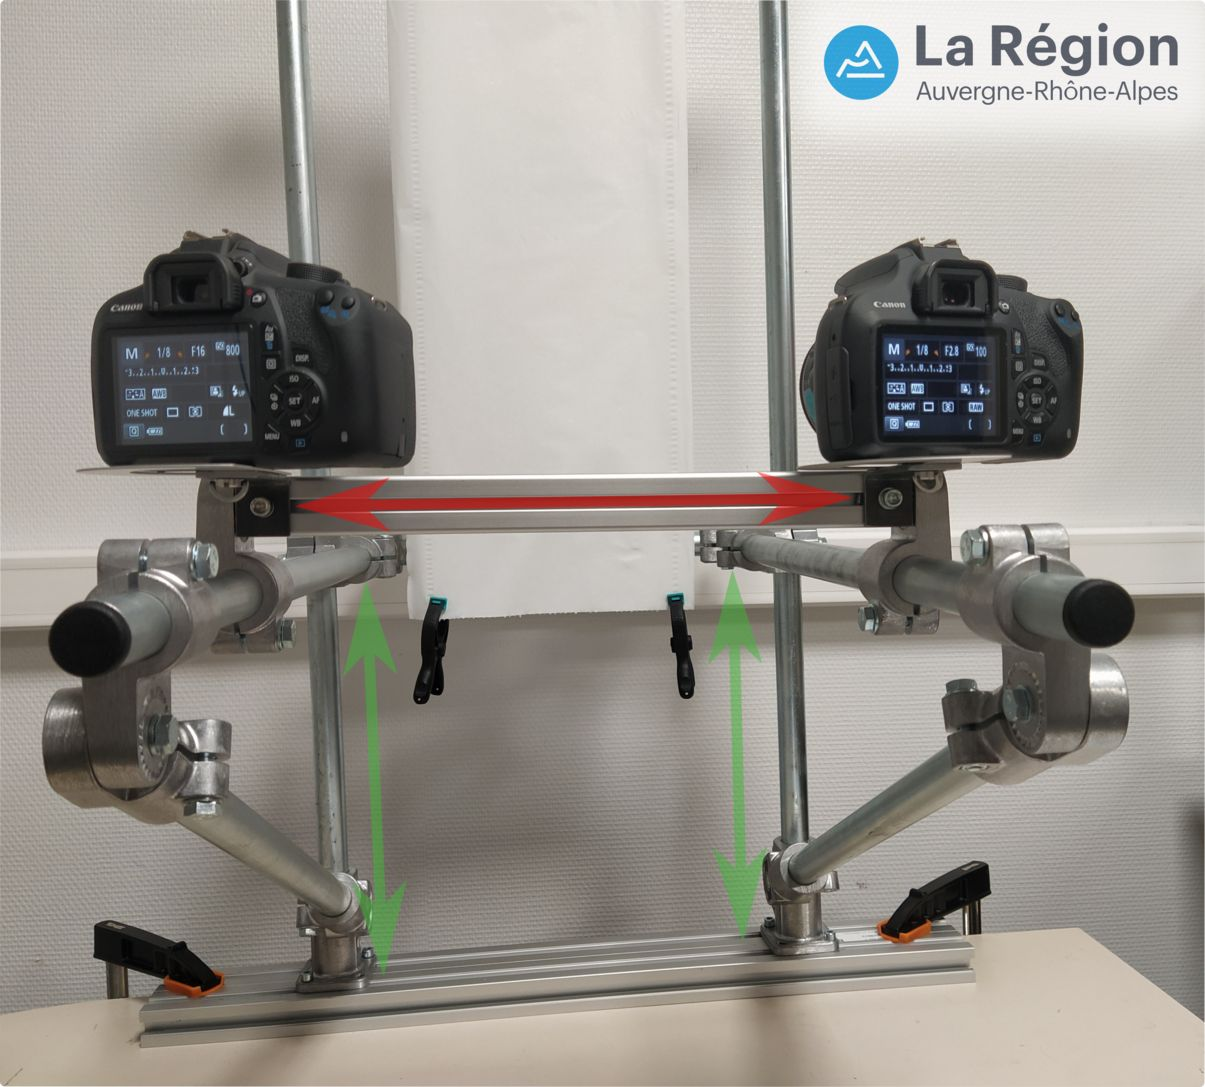
\includegraphics[width=\linewidth]{dispositif_statique_01.jpg}
				\caption{}
			\end{subfigure}
			\begin{subfigure}[b]{.52\linewidth}
				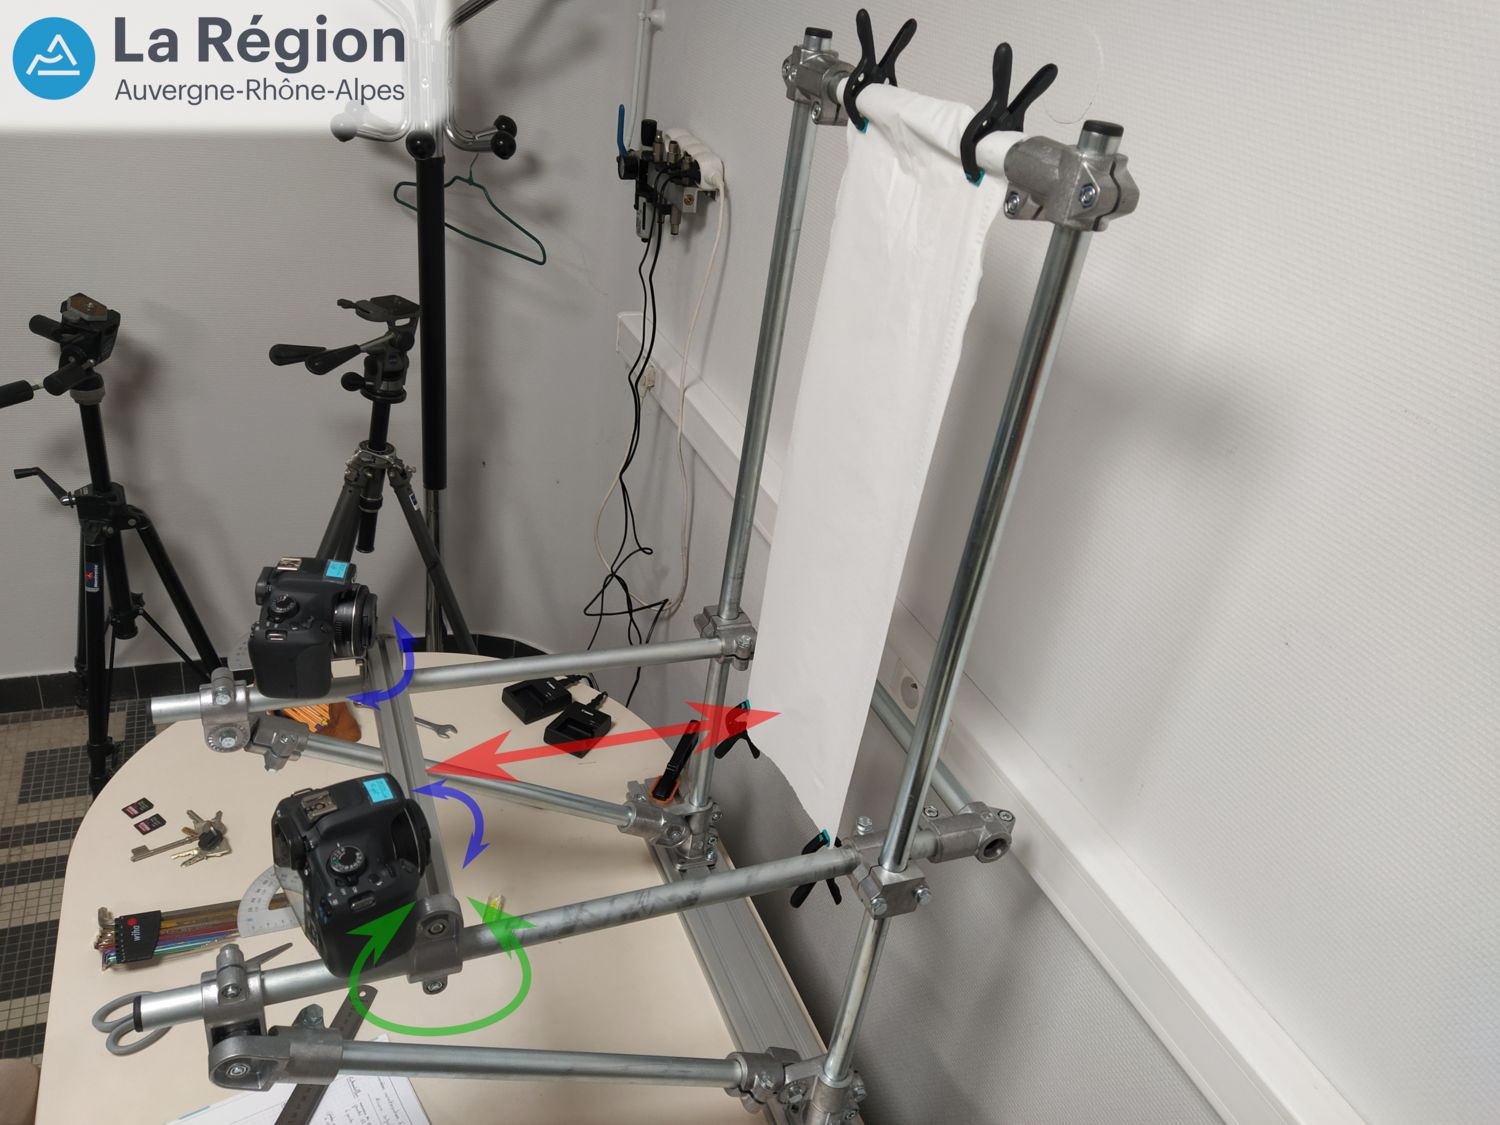
\includegraphics[width=\linewidth]{dispositif_statique_02.jpg}
				\caption{}
			\end{subfigure}
		\caption{\label{fig:dispositif_statique}Dispositif de caractérisation par stéréovision pour des applications en statique. Les degrés de liberté du dispositif sont représentés par les flèches de couleurs et présentés dans le paragraphe associé.}
		\end{figure}
		\\Actuellement, il n'est pas évident d'être précis dans la connaissance de ces réglages et certaines améliorations pourraient voir le jour dans les prochains mois. La méthode actuelle consiste à mesurer à l'aide d'un réglet les différentes longueurs. Des rapporteurs sont également fixés aux supports des appareils photographiques afin d'estimer de manière relativement correcte les angles de chacune des caméra définissant les champs horizontaux. Il est a noter qu'il est possible de connaître de manière assez précise la position et l'orientation de chacune des caméra par une méthode numérique. Il suffit pour cela de prendre un cliché d'une mire dont la position est parfaitement connue dans l'espace : si les deux caméras sont calibrés alors il est possible de remonter à leurs positions respectives. Dans cette condition, il est important de connaître parfaitement la position de la mire sur le dispositif expérimental.

\section{Travaux numériques réalisés}
	Bien que le montage soit fonctionnel, le projet se destine essentiellement à du traitement numérique. Le choix du langage de programmation Python a été fait, puisqu'il s'agit d'un langage très courant, de haut niveau et donc relativement facile à utiliser avec énormément de ressources. De plus, la librairie IPSDK développée par \href{https://www.reactivip.com/fr/accueil/}{Reactiv'IP} sera utilisée pour le traitement d'image et possède une implémentation en Python.
	\\Le travail numérique consiste en plusieurs tâches qui peuvent être elles-mêmes regroupées en différentes catégories selon les objectifs. Pour cette raison, une librairie associée au projet a été créée. Cette librairie présente différents modules permettant de répondre à différentes problématiques. Une présentation plus détaillée est faite dans les prochains paragraphes.
	\subsection{Librairie Python ds3dlive}
		\begin{figure}\centering
			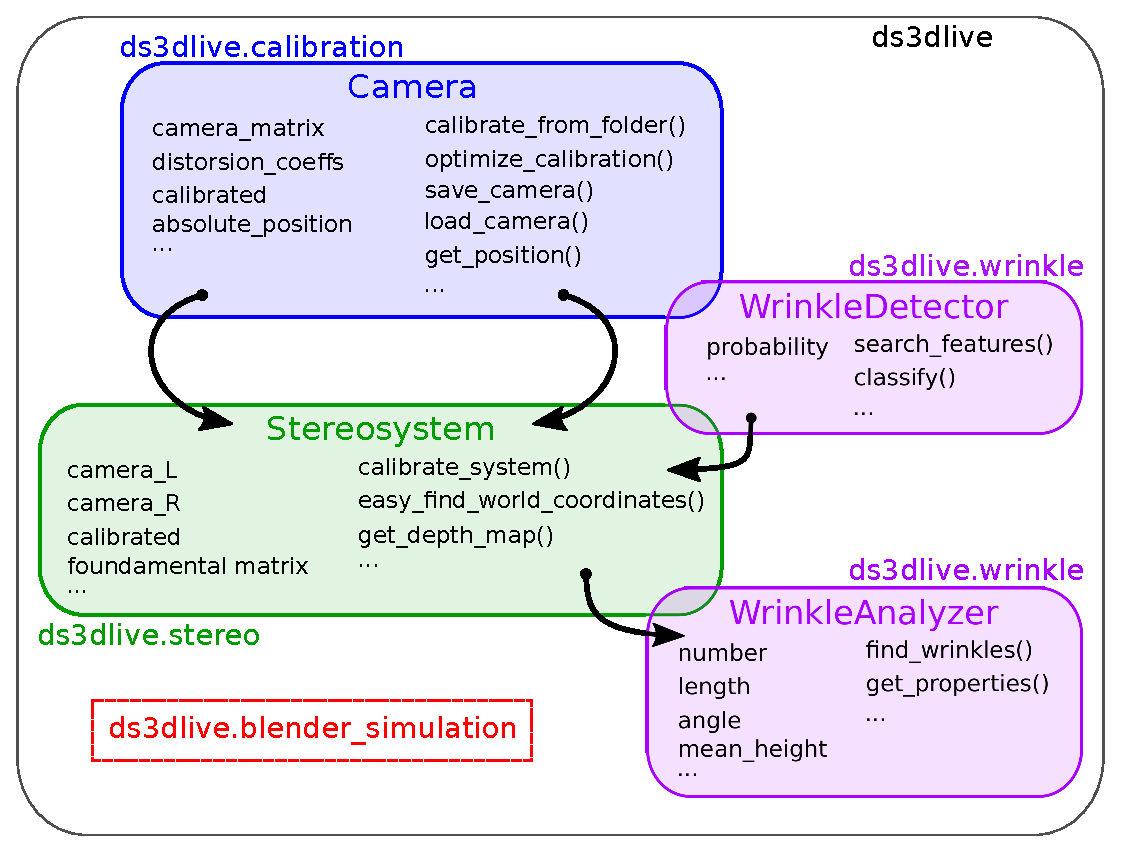
\includegraphics[width=.7\linewidth]{logigramme.eps}
			\caption{\label{fig:logigramme}Diagramme fonctionnel de la librairie ds3dlive. La librairie est constituée de plusieurs modules (calibration, stereo, ...) qui génère des objets de différentes classes (Camera, Stereosytem, ...) interagissant entre eux.}
		\end{figure}
		La librairie développée en Python dans ce projet est simplement nommée par le nom du projet : ds3dlive. Cette librairie est en cours de développement et n'est pas encore distribuable. Le travail de développement se fait par contre par l'intermédiaire de l'outil très populaire Git grâce à un workflow de type "gitflow". Afin de détailler cette dernière phrase : plusieurs versions du programme existent. Une version stable et fonctionnelle est toujours disponible. En parallèle, une branche du même programme en cours de développement est en perpétuelle évolution. Lorsque l'occasion le permet, la version stable est mise à jour par la version en développement. Chaque ajout ou modification d'une fonctionnalité est traitée à part et est testée avant d'être envoyée sur la version de développement. A chaque fois qu'une mise à jour est faite, des tests unitaires sont réalisés afin de prévenir des problèmes pouvant intervenir suites aux modifications effectuées.
		\\La librairie possède des modules dont certains sont déjà en cours de développement et bien avancés :
		\begin{description}
			\item[calibration :] Il s'agit de la librairie qui gère les caméras / APN. Ce module permet de les calibrer, de sauvegarder leurs propriétés, de les charger mais aussi d'interagir directement avec les images fournies par le système (corriger la distorsion par exemple). Afin de permettre tout cela, le module génère des objets "Camera".
			\item[stereo :] Ce module est basé sur l'objet "Stereosystem" qui est formé par deux objets "Camera". Le module se charge de définir les contraintes épipolaires associé au système de stéréovision et de connaître les positions exactes des caméras / APN afin d'être capable de situer des points dans l'espace (en cours de développement).
			\item[blender\_simulation :] Ce module n'est pas destiné à être utilisé en console ou avec une interface graphique. Il est destiné à créer un modèle 3D sur le logiciel Blender et s'ouvre donc depuis la console Python intégrée dans le logiciel.
			\item[wrinkle :] Le module a pour objectif de détecter de manière automatique la présence de plis sur le papier (développement à faire) et de caractériser dimensionnellement les plis lorsqu'ils sont détectés et que l'information 3D est accessible (développement en cours).
		\end{description}
		La librairie est accessible sur le site internet \href{https://github.com/}{GitHub} sous la forme d'un projet privé détenu par le compte personnel "MaximeTeil". Il est possible de partager ce répertoire entre trois collaborateurs (deux autres comptes donc). A la demande de chacun, un accès peut être ouverts aux partenaires du projet. La limite du nombre de collaborateurs peut entraîner des accès temporaires et non permanents.
		\\Une discussion peut être ouverte concernant le passage du répertoire en mode "public". Ceci permettrait à tout le monde d'accéder au projet et de participer aux différentes tâches. En contrepartie, la confidentialité des travaux ne serait plus maintenue.
	
	\subsection{Calibration de caméra / APN}
		Le module de calibration de caméra est adapté à la création d'objets de la classe "Camera". Ces objets ont pour objectif de stocker l'ensemble des propriétés intrinsèques à la caméra associée et de proposer un ensemble de méthodes pour traiter les données efficacement et faciliter les tâches de l'utilisateur. La création d'un objet de la classe Camera peut se faire sans aucune information. Cela aura pour conséquence de générer une caméra dont les propriétés sont toutes nulles par défaut. Une manière de mesurer et calculer les propriétés de la caméra est de la calibrer selon la théorie présentée dans l'annexe \ref{annexe:calibration}.
		\\La méthode de calibration consiste à prendre plusieurs clichés d'une mire bien connue, prise sous différents angles. Cette mire est constituée de zones à très fortes différences de contraste permettant ainsi de sélectionner de manière automatique et précise des points dont les positions sont connues. L'utilisation de cette mire permet de créer une table de correspondance entre la position des points réels dans l'espace et la position des points images associés dans les images obtenues. La mire utilisée actuellement dans le projet est de type "damier" : chaque contact entre les carrés noirs sont de points faciles à détecter automatiquement. La position des points est déterminée par la taille des carrés, le nombre de lignes et le nombre de colonnes du damier. Un script \LaTeX\ a été implémenté afin de générer automatiquement au damier au format PDF : il suffit de rentrer en variable le nombre de lignes, colonnes et la taille souhaitée des carrés. Les exemples donnés ici présentent une mire de \num{7} lignes, \num{11} colonnes et dont les carrés ont des côtés de \SI{20}{\milli\meter}. Un cliché permettant de calibrer une caméra est montré sur la figure \ref{fig:mire}.
		\begin{figure}\centering
			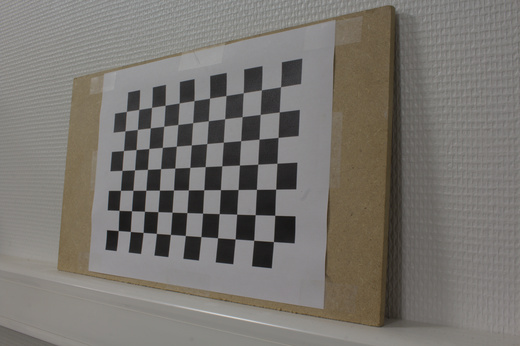
\includegraphics[width=.5\linewidth]{IMG_8853_small.jpg}
			\caption{\label{fig:mire}Prise de vue permettant de calibrer une caméra avec une mire de type "damier" de \num{7x11} et des carrés de \SI{20}{\milli\meter}.}
		\end{figure}
		\\En fonction du nombre d'images acquises ($n$) et du nombre de points constituant la mire ($p$), un système d'équations linéaires en $\overline{\overline{P}}$ peut être obtenu :
		\begin{equation}
			\forall (n, p) \in (\mathbb{N}_+^*)^2, \qquad \overline{q}_{n, p} \sim \overline{\overline{P}}_n \cdot \overline{Q}_{n, p}
		\end{equation}
		Puisque les images présentent obligatoirement du bruit et que le problème est surdimensionné, la résolution de ce système de se fait au sens des moindres carrés. Une décomposition en valeurs singulières permet de trouver les éléments constituant les matrices $\overline{\overline{P}}_n$ qui minimisent l'erreur quadratique sur le système d'équations.
		\\La connaissance des matrices de projection $\overline{\overline{P}}_n$ donne accès aux matrices de calibration $\overline{\overline{K}}_n$ (voir annexe \ref{annexe:calibration} au besoin). La matrice de calibration de la caméra est déterminée comme étant la moyenne arithmétique des matrices de calibration pour chaque prise de vue :
		\begin{equation}
			\forall n \in \mathbb{N}_+^*, \quad \overline{\overline{K}} = \cfrac{\sum_n \overline{\overline{K}}_n}{n}
		\end{equation}
		Le module permet également de déterminer la pose lorsque la caméra a été déplacée. En effet, ayant connaissance des paramètres intrinsèques à la caméra avec la matrice de calibration, il est possible de déterminer les paramètres extrinsèques pour établir la matrice de projection. Une solution pour permettre cela est donc une nouvelle fois d'utiliser la mire pour être capable de déterminer la position et l'orientation de la caméra par rapport à cette mire. Il peut être envisagé de placer des autocollants sur le montage afin d'assurer une pose toujours relative au même repère. Dans ce cas, il faut s'assurer d'avoir au moins \num{3} points de mire (la méthode s'appelle d'ailleurs la méthode des 3 points).
		\\Enfin, la connaissance des coefficients de distorsion lors de la phase de calibration permet au module d'utiliser les propriétés de la caméra pour déformer l'image acquise afin de corriger les déformations liées à la distorsion. Cela est très important pour des applications de métrologie.
		\\Les algorithmes permettant la calibration des caméras sont basés sur la librairie Python d'OpenCV, qui possède un module de calibration 3D. Cette librairie est surtout utilisée pour détecter automatiquement et très précisément les points de mire et pour approximer efficacement les coefficients de distorsion. Dans la condition où ces deux outils pourraient être développés dans la librairie IPSDK, l'ensemble de ce module de calibration pourrait être implémenté avec IPSDK.
	
	\subsection{Système de stéréovision}
		Le module de stéréovision est constitué d'une classe "Stereosystem" qui est construit à partir de deux objets de la classe Camera. Les propriétés de chacune des caméras sont utilisées pour définir la contrainte épipolaire du système et être capable de situer un point dans l'espace à partir des points images associés sur chacun des capteurs. Ce module a finalement deux objectifs principaux :
		\begin{itemize}
			\item \^Etre capable d'utiliser la contrainte épipolaire pour retrouver des points stéréocorrespondants ;
			\item \`A partir des points stéréocorrespondants, être capable de déterminer la position du point objet dans le repère monde (ou dans le repère caméra).
		\end{itemize}
		\paragraph{Géométrie épipolaire -}
			La contrainte épipolaire est la contrainte qui permet de dire que si l'on s'intéresse à un point image sur une des deux images du système alors le point image associé dans l'autre image est placé sur une droite (dont on est capable de calculer l'équation). La position sur cette droite est déterminée par la profondeur du point objet par rapport au repère caméra : la position dépend donc de $Z^C$ (voir annexe \ref{annexe:calibration}). La contrainte épipolaire peut être définie par l'intermédiaire d'une matrice \num{3x3} $\overline{\overline{F}}$, appelée matrice fondamentale, grâce à la relation suivante :
			\begin{equation}
				\overline{q_2}^T \cdot \overline{\overline{F}} \cdot \overline{q_1} = 0
			\end{equation}
			où $\overline{q_1}$ et $\overline{q_2}$ sont les coordonnées dans le repère des pixels des points images sur chacune des images.
		\paragraph{Géométrie épipolaire calibrée -}
			Dans le cas où les matrices de calibration des caméras sont bien connues, il est possible de déterminer la contrainte épipolaire uniquement avec les paramètres extrinsèques des caméras (leurs positions et orientations) en travaillant dans les repères images et non plus dans les repères des pixels. La contrainte devient alors, en utilisant les termes de l'annexe \ref{annexe:calibration} :
			\begin{equation}
				\overline{q_{i2}}^T \cdot \overline{\overline{E}} \cdot \overline{q_{i_1}} = 0
				\quad\text{avec}\quad
				\overline{\overline{E}} \sim \overline{\overline{K_2}}^T \cdot \overline{\overline{F}} \cdot \overline{\overline{K_1}} \sim
				\overline{\overline{R_2}} \cdot \overline{\overline{[\overline{t_1} - \overline{t_2}]_\times}} \cdot \overline{\overline{R_1}}^T
			\end{equation}
			Ici, la notation matricielle du produit vectoriel est utilisée :
			\begin{equation}
				\overline{\overline{[\overline{a}]_\times}} = \begin{pmatrix}
					0 & -a_3 & a_2\\a_3 & 0 & -a_1\\-a_2 & a_1 & 0
				\end{pmatrix}
			\end{equation}
		\paragraph{Reconstruction 3D -}
			\`A partir des paramètres intrinsèques et extrinsèques des deux caméras, il est possible de définir leur matrice de projection, respectivement $\overline{\overline{P_1}}$ et $\overline{\overline{P_2}}$. Lorsque deux points $\overline{q_1}$ et $\overline{q_2}$ sont stéréocorrespondants, il est possible de reconstruire le point objet $\overline{Q}$ associé dans le repère monde par l'intermédiaire du système suivant, linéaire en les coefficients de $\overline{Q}$ :
			\begin{equation}
				\left\{\begin{array}{l}
					\overline{\overline{P_1}} \cdot \overline{Q} \sim \overline{q_1} \\
				\overline{\overline{P_2}} \cdot \overline{Q} \sim \overline{q_2}
				\end{array}\right.
			\end{equation}
		\paragraph{Exemple de mesure 3D\\}
			\begin{figure}\centering
				\begin{subfigure}[c]{.48\linewidth}
					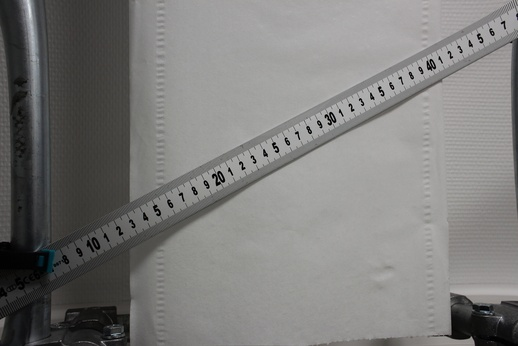
\includegraphics[width=\linewidth]{regletL_undistorted_small.jpg}
					\caption{vue de gauche}
				\end{subfigure}
				\begin{subfigure}[c]{.48\linewidth}
					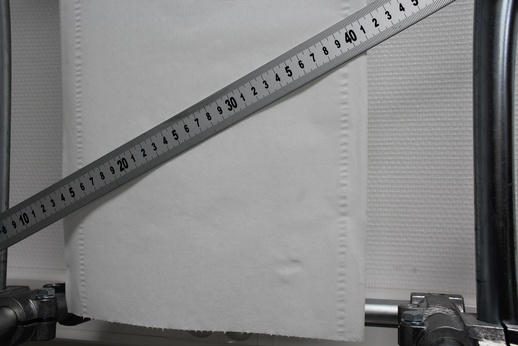
\includegraphics[width=\linewidth]{regletR_undistorted_small.jpg}
					\caption{vue de droite}
				\end{subfigure}
				\caption{\label{fig:exemple_reconstruction_3D}Prise de vue stéréoscopique d'un réglet afin de vérifier la mesure 3D. Les images présentées sont corrigées de la distorsion.}
			\end{figure}
			Considérons la prise de vue stéréoscopique présentée sur la figure \ref{fig:exemple_reconstruction_3D}. Un réglet a été placé dans le champ de vision des deux caméras. Nous allons tenter de mesurer une longueur de \SI{1}{\milli\meter} sur ce réglet. Pour cela, les coordonnées des extrémités de deux lignes adjacentes sur le réglet vont être prélevées manuellement : nous avons alors, pour chaque trait, $\overline{q_1}$ et $\overline{q_2}$. La calibration des caméras a été faite et le système stéréoscopique a également été calibré : nous avons $\overline{\overline{P_1}}$ et $\overline{\overline{P_2}}$. La table \ref{tab:coordonnees_exemple} indique les coordonnées retrouvées manuellement pour les traits de réglet de \SI{297}{\milli\meter} et \SI{298}{\milli\meter} ainsi que les coordonnées calculées dans le repère monde. La norme mesurée du vecteur reliant les deux traits de réglet dans le repère monde est de \SI{.959}{\milli\meter} pour une valeur théorique de \SI{1}{\milli\meter}. Cela représente une erreur relative de \SI{4.09}{\percent}.
			\begin{table}\centering
				\begin{tabular}{c@{\hspace{3em}}c@{\hspace{3em}}c@{\hspace{3em}}c}
					\hline
					Trait de réglet & $\overline{q_1}$ & $\overline{q_2}$ & $\overline{Q}$ \\\hline
					\SI{297}{\milli\meter} & $\begin{pmatrix}3227.14\\1107.86\end{pmatrix}$ & $\begin{pmatrix}2234.89\\962.97\end{pmatrix}$ & $\begin{pmatrix}98.90\\15.46\\10.09\end{pmatrix}$ \vspace{.5em} \\
					\SI{298}{\milli\meter} & $\begin{pmatrix}3237.61\\1101.94\end{pmatrix}$ & $\begin{pmatrix}2245.79\\956.81\end{pmatrix}$ & $\begin{pmatrix}99.75\\15.02\\10.09\end{pmatrix}$ \\\hline
				\end{tabular}
				\caption{\label{tab:coordonnees_exemple}Prise manuelle des coordonnées dans les repères des pixels pour chaque trait de réglet étudié.}
			\end{table}
			\\L'erreur relative semble rester aux alentours de cette valeur lorsque le même exercice est réalisé sur des longueurs plus grandes ( \textit{i.e.} de l'ordre de plusieurs centimètres). Cette erreur peut provenir :
			\begin{itemize}[label=$\rightarrow$]
				\item Du bruit présent dans les images ;
				\item De la précision de la calibration et de la correction de la distorsion ;
				\item D'une erreur de lecture humaine sur les points images ;
				\item De la précision de la mire.
			\end{itemize}
			
	
	\subsection{Simulation 3D}
		Afin de commencer les travaux numériques sur le traitements d'images et de permettre une mise en place facilitée du dispositif expérimental, des simulations peuvent être réalisées grâce au logiciel de modélisation 3D Blender.
		\begin{figure}\centering
			\begin{subfigure}[c]{.48\textwidth}
				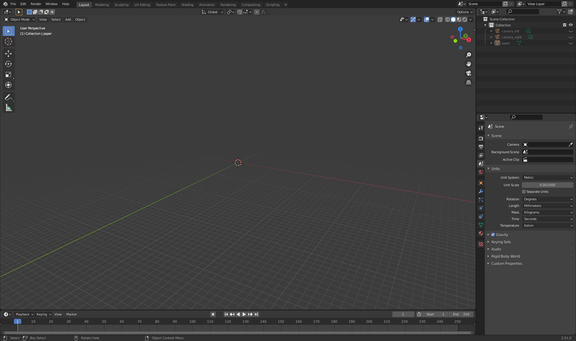
\includegraphics[width=\textwidth]{screen_0_resized.png}
				\caption{Création du projet Blender}
			\end{subfigure}\hfill
			\begin{subfigure}[c]{.48\textwidth}
				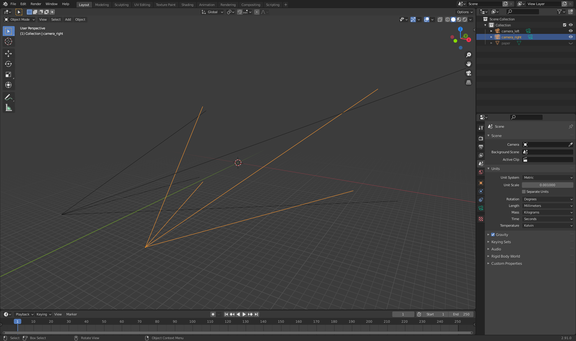
\includegraphics[width=\textwidth]{screen_2_resized.png}
				\caption{Ajout des caméras}
			\end{subfigure}\\
			\begin{subfigure}[c]{.48\textwidth}
				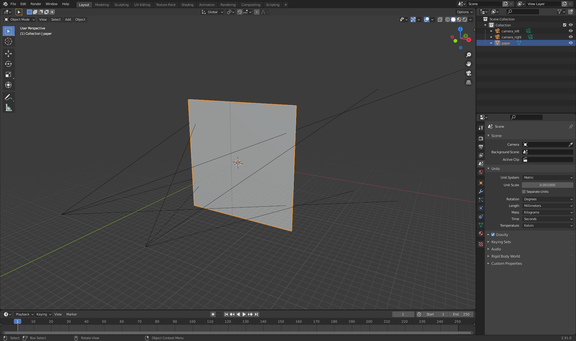
\includegraphics[width=\textwidth]{screen_3_resized.png}
				\caption{Ajout du papier avec pli vertical}
			\end{subfigure}\hfill
			\begin{subfigure}[c]{.48\textwidth}
				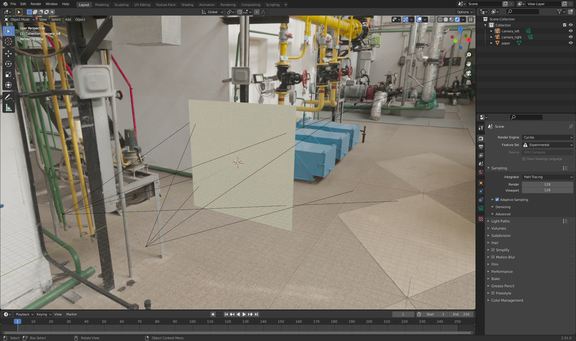
\includegraphics[width=\textwidth]{screen_4_resized.png}
				\caption{Ajout d'un "monde" réaliste}
			\end{subfigure}\\
			\begin{subfigure}[c]{.48\textwidth}
				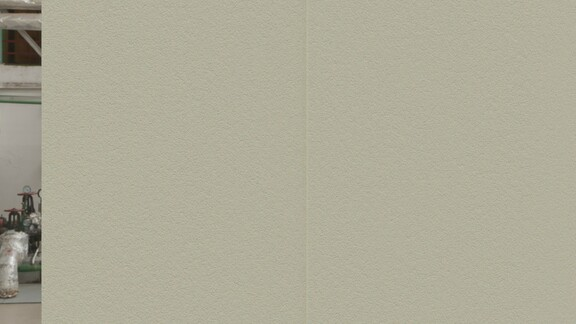
\includegraphics[width=\textwidth]{view_0_resized.jpg}
				\caption{Acquisition de l'image de gauche}
			\end{subfigure}\hfill
			\begin{subfigure}[c]{.48\textwidth}
				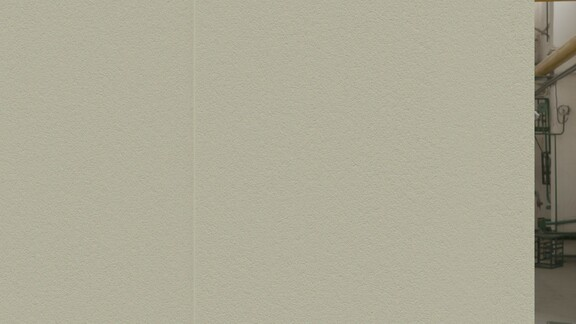
\includegraphics[width=\textwidth]{view_1_resized.jpg}
				\caption{Acquisition de l'image de droite}
			\end{subfigure}
			\caption{\label{fig:blender}Utilisation "graphique" de Blender dans ce projet}
		\end{figure}
		\\La figure \ref{fig:blender} illustre les différentes étapes permettant de simuler le dispositif expérimental ainsi que le papier avec un pli vertical. Cela peut être réalisé par l'intermédiaire de l'interface graphique du logiciel mais il a été fait le choix de mener l'ensemble de cette procédure de manière automatique grâce à un script Python, qui peut être lu par le logiciel Blender. Un module Python a été créé pour générer des fonctions utiles à ce projet. Le principe consiste à générer un fichier de paramètres au format "tsv", par exemple dans un tableur numérique, puis de lire les paramètres de ce fichier dans les fonctions du module associé. L'annexe A présente le code interprété par le logiciel Blender. Les annexes B et C représentent quant à elles, respectivement, un exemple de fichier de paramètres au format tsv et le module qui regroupe l'ensemble des fonctions pouvant être utiles au projet.
		\\\`A l'instant où ces lignes sont écrites, la simulation ne permet de générer que des plis dans la direction verticale. Les plis sont générés selon un profil gaussien décrit par l'équation (\ref{eq:gaussienne}). Ce profil est déterminé selon deux paramètres : la hauteur du pli et sa largeur à mi-hauteur. Un troisième paramètre permet de situer le pli sur le matériau papier (c'est-à-dire selon l'axe horizontal). Enfin, un quatrième paramètre définit la résolution du maillage pour être plus ou moins précis dans la forme donnée au profil gaussien.
		Les paramètres qui rentrent en considération sont présentés dans la table \ref{tab:parametres_blender}.
		\begin{table}
			\begin{tabular}{|r @{$\quad\rightarrow\quad$} p{0.8\linewidth}|}
				\hline
				\multicolumn{2}{|c|}{Paramètres propres au dispositif}  \\ \hline
				& Distance caméra 1 / caméra 2 \\
				& Distance caméras / papier \\
				& Angles des caméras \\
				& Largeur du papier \\
				& Largeur, hauteur, position et résolution du pli \\
				& Longueurs focales des caméras \\
				& \'Eclairages \\
				& Autres à venir... \\ \hline
				\multicolumn{2}{|c|}{Paramètres physiques} \\ \hline
				& Texture prédéfinie (pas obligatoire) \\
				& Rugosité \\
				& Effet "subsurface" (transmission partielle de l'éclairage sur l'épaisseur du matériau avec potentielle modification des couleurs) \\
				& Autres à venir... \\ \hline
				\multicolumn{2}{|c|}{Paramètres de rendu} \\ \hline
				& Moteur de rendu \\
				& Insertion du monde dans la scène \\
				& Type et méthodes de calcul \\
				& Taille et format des images de sortie \\
				& Nombre d'images moyennées \\
				& Gestion des sauvegardes \\
				& Autres à venir... \\ \hline
			\end{tabular}
			\caption{\label{tab:parametres_blender}Paramètres qui rentrent en considération dans la simulation Blender}
		\end{table}
	
	\subsection{Caractérisation de plis par Alicona Infinite Focus}
		\label{section:Alicona}
		Dans le but de connaître les dimensions caractéristiques d'un pli, une analyse microscopique a été menée grâce à la machine Alicona Infinite Focus. Une carte topographique centrée sur une zone de dimensions $\SI{35 x 2.5 x 1}{\milli\meter}$ (dimensions selon, respectivement, l'axe, la largeur et la hauteur du pli) autour du pli a été calculée, ce qui permet de mailler la surface du papier et de déterminer certaines caractéristiques.
		\begin{figure}\centering
			\begin{subfigure}[b]{.54\linewidth}
				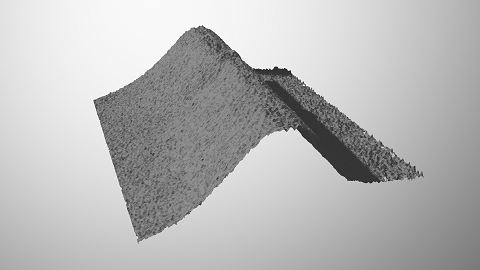
\includegraphics[width=\linewidth]{pli_01_3d_small.png}
				\caption{Topographie 3D}
			\end{subfigure}
			\begin{subfigure}[b]{.44\linewidth}
				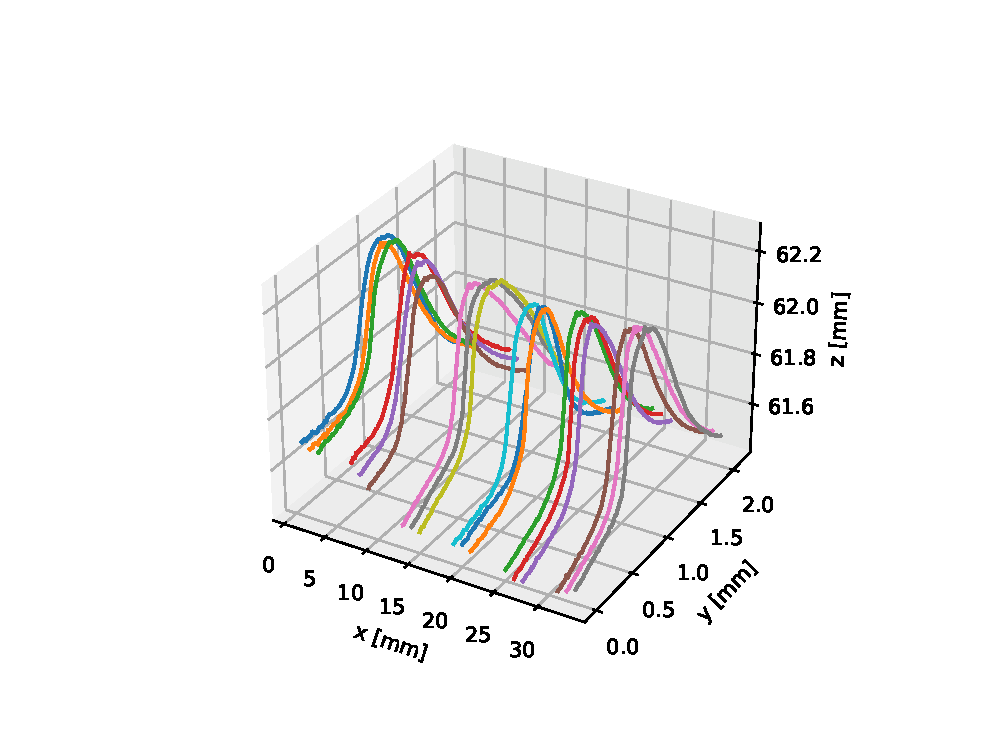
\includegraphics[width=\linewidth]{profiles.eps}
				\caption{Analyse de profils transversaux}
			\end{subfigure}
			\caption{\label{fig:caracterisation_pli}Caractérisation géométrique d'un pli}
		\end{figure}
		\\La figure \ref{fig:caracterisation_pli} montre une représentation 3D de la topographie au niveau du pli ainsi que les courbes définissant \num{18} profils transversaux qui permettent de moyenner les caractéristiques géométriques sur la longueur de \SI{35}{\milli\meter}. Deux caractéristiques ont été calculées :
		\begin{itemize}[label=$\Rightarrow$]
			\item La hauteur du pli (selon la direction $z$) : $707 \pm 74$~\si{\micro\meter} ;
			\item La largeur du pli à mi hauteur (selon la direction $y$) : $680 \pm 167$~\si{\micro\meter}.
		\end{itemize}
		Le pli analysé a été généré lors de la formation sur la machine pilote et a été qualifié de "relativement grossier" dans le sens où il s'agit ici d'un pli dont la largeur semble relativement importante au regard de ceux qui ont été observés jusqu'à présent.
		\\L'observation de la vue 3D et des profils transversaux nous entraîne à penser que le profil transversal d'un pli pourrait être décrit localement par une fonction gaussienne, pour laquelle il est facile de trouver l'équation (\ref{eq:gaussienne}) en fonction de sa position centrale $X$, de la largeur à mi-hauteur $l_{1/2}$ et de l'amplitude du pic $A$ :
		\begin{equation}\label{eq:gaussienne}
		\left\{
		\begin{array}{l}
		\mathbb{R} \mapsto \mathbb{R} \\
		x \rightarrow \cfrac{A}{\sigma\sqrt{2\pi}}\ e^{-\cfrac{(x - X)^2}{2\sigma^2}} \qquad \text{avec}\qquad 
		\sigma = \cfrac{l_{1/2}}{2\sqrt{2\ln2}}\ \approx\ \num{0.425} \cdot l_{1/2}
		\end{array}\right.
		\end{equation}
		D'autres observations sur Alicona Infinite Focus sont prévues dans la suite pour caractériser des plis dont les dimensions sont plus caractéristiques de celles des plis qui se forment sur la machine pilote.


\section{Gestion du projet}
	\subsection*{Perspectives}
		Certaines tâches n'ont pas encore été traitées et vont l'être dans les prochains mois :
		\begin{itemize}[label=$\rightarrow$]
			\item Traitement des images avec la librairie IPSDK.
			\item Développement d'un détecteur de plis : la méthode SIFT pourrait être utilisée (voir annexe \ref{annexe:sift}) avec la librairie IPSDK.
			\item Optimisation de la mesure 3D avec la triangulation \cite{hartley_triangulation_1997}.
		\end{itemize}
	
	\subsection*{Gestion}
		\begin{itemize}[label=$\rightarrow$]
			\item Communication régulière sur les réseaux LinkedIn et ResearchGate à partir de maintenant.
			\item Dépenses réalisées en matériel : \num{1612.85} \euro.
			\item Collaborations sur le projet GitHub ? Privé / public ?
		\end{itemize}
		


\bibliographystyle{unsrt}
\bibliography{biblio}

\appendix
\newpage
\null
\begin{center}
	\vfill\Huge
	Annexes
	\vfill\null
\end{center}
\newpage

\section{Calibration des systèmes optiques - Théorie}
	\label{annexe:calibration}
	Le modèle de sténopé est présenté ici. Nous allons voir comment calibrer une caméra en tenant compte de ce modèle.
	\subsection*{Modèle de sténopé - Repères dans l'espace}
		Quatre repères sont nécessaires pour bien interprété le modèle de sténopé et pouvoir situer un point dans l'espace. Les repères choisis sont les suivants :
		\begin{itemize}[label=$\rightarrow$]
			\item Repère monde : $Q\left( X, Y, Z \right)$. Repère fixe dans l'espace, qui est couramment utiliser en sciences physiques.
			\item Repère caméra : $Q^C\left( X^C, Y^C, Z^C \right)$. Repère qui a pour origine le centre de projection de la caméra et dont l'axe optique porte et oriente l'axe selon $Z^C$. $X^C$ et $Y^C$ sont orientés selon les axes des pixels sur le capteur de la caméra (respectivement, axe horizontal de gauche à droite et axe vertical de haut en bas).
			\item Repère image : $q_i\left( x, y \right)$. Repère à deux dimensions dont l'origine est le point principal (intersection entre l'axe optique et le plan image). Les axes déterminant $x$ et $y$ sont ceux définissant les axes $X^C$ et $Y^C$, respectivement, dans le repère caméra.
			\item Repère des pixels : $q\left( u, v \right)$. Repère identique au repère image à la différence près que l'origine est le coin supérieur gauche de l'image et les dimensions sont exprimées en pixels.
		\end{itemize}
	La figure \ref{fig:stenope_repere} illustre chacun de ces repères. Considérant un point dans l'espace à trois dimension $Q$, il est possible de déterminer les coordonnées de sa projection $q$ dans le plan image - dans un repère à deux dimension donc. L'étude de la projection de points dans l'espace 3D dans un espace 2D nous amène à travailler avec les coordonnées homogènes. En présence de coordonnées homogènes, le symbole "$\sim$" correspond à une égalité vectorielle définie à un facteur près :
	\begin{equation}
		\exists s\in\mathbb{R}, \qquad \overline{q}\sim\overline{Q} \quad \Leftrightarrow \quad s\overline{q} = \overline{Q}
	\end{equation}
	\begin{figure}[h]\centering\scriptsize
		\begin{tikzpicture}[scale=3.]
			\coordinate (Oc) at (0, 0) node[left, blue] {caméra};
			\coordinate (Oi) at (35:4em);
			\coordinate (Om) at (28:8.5em);
			% Monde
			\draw[very thick, -stealth, blue] (Om) node[left] {monde} -- ++(10: 1em) node[right] {$X$};
			\draw[very thick, -stealth, blue] (Om) -- ++(90: 1em) node[left] {$Y$};
			\draw[very thick, -stealth, blue] (Om) -- ++(-35: .8em) node[right] {$Z$};
			% point Q
			\draw[thick] (Oc) -- ++(12:8em) coordinate (Q) node {$\bullet$} node [above right] {$Q$};
			% Image
			\begin{scope}[scale=1.8, shift=(Oi)]
				\filldraw[gray!30] (-10:-1.5em)++(-90:-1em) coordinate (Op) -- ++(-10:3em) -- ++(-90:2em) -- +(-10:-3em) -- cycle;
				% Pixels
				\draw[very thick, -stealth, blue] (Op) -- ++(-10:.4em) node[below right] {$u$};
				\draw[very thick, -stealth, blue] (Op) -- ++(-90: .4em) node[below left] {$v$};
				\draw (Op) node[left, blue] {pixels};
			\end{scope}
			\draw[very thick, -stealth, blue] (Oi) -- ++(-10: 1em) node[below right] {$x$};
			\draw[very thick, -stealth, blue] (Oi) -- ++(-90: 1em) node[below left] {$y$};
			\draw (Oi) node[above left, blue] {image};
			% Point q
			\draw[thick, dashed, gray] (Oc)++(12:4.5em) coordinate (q) -- ++(12:1.6em);
			\draw[thick] (Oc) -- (q) node {$\bullet$} node [above right] {$q$};
			% axe optique
			\draw[dashed] (Oc) -- (Oi);
			% Caméra
			\draw[very thick, -stealth, blue] (Oc) -- ++(-10: 1em) node[below right] {$X^C$};
			\draw[very thick, -stealth, blue] (Oc) -- ++(-90: 1em) node[below left] {$Y^C$};
			\draw[very thick, -stealth, blue] (Oc) -- ++(35: 1em) node[left] {$Z^C$};
		\end{tikzpicture}
		\caption{\label{fig:stenope_repere}Repère dans les différents espaces pour le modèle de sténopé.}
	\end{figure}
	\\L'objectif de la calibration est d'être capable de définir mathématiquement la relation qui relie la position d'un point dans l'espace ($Q$ ici) à sa projection sur l'image ($q$ ici). On cherche donc une matrice $\overline{\overline{P}}$ (dimensions 3 par 4), qui relie $\overline{q}$ (dimension 3) à $\overline{Q}$ (dimension 4) :
	\begin{equation}
		\begin{pmatrix}
			u\\v\\1
		\end{pmatrix} \sim \overline{\overline{P}}\begin{pmatrix}
			X\\Y\\Z\\1
		\end{pmatrix}
		\qquad\Leftrightarrow\qquad
		\overline{q} \sim \overline{\overline{P}} ~ \overline{Q}
	\end{equation}
	La matrice $P$ est appelée la matrice de projection de la caméra.
	\paragraph{Passage du repère caméra au repère image\\}
		Par définition et notion d'optique géométrique, la distance focale $f$ correspond à la distance entre le centre de projection du système optique et le point principal, qui est à la fois sur l'axe optique et sur le plan image. Cela veut dire que la distance focale correspond à la distance entre l'origine du repère caméra et l'origine du repère image.
		\\On montre géométriquement (théorème de Thalès):
		\begin{equation}
			\left\{ \begin{array}{l}
				x\ =\ f\cfrac{X^C}{Z^C}\vspace{.7em}\\
				y\ =\ f\cfrac{Y^C}{Z^C}
			\end{array}\right.
			\quad\Leftrightarrow\quad
			\begin{pmatrix}
				x\\y\\1
			\end{pmatrix} \sim \begin{pmatrix}
				f & 0 & 0 & 0\\
				0 & f & 0 & 0\\
				0 & 0 & 1 & 0
			\end{pmatrix}\begin{pmatrix}
				X^C\\Y^C\\Z^C\\1
			\end{pmatrix}
			\quad\Leftrightarrow\quad
			\overline{q_i} \sim \begin{pmatrix}
			f & 0 & 0 & 0\\
			0 & f & 0 & 0\\
			0 & 0 & 1 & 0
			\end{pmatrix} \overline{Q^C}
		\end{equation}
	\paragraph{Passage du repère image au repère des pixels\\}
		Le passage entre ces deux repères se fait par l'intermédiaire d'une translation (pour placer l'origine sur un coin de l'image) et d'un changement d'unité (pour passer d'une longueur métrique à une longueur en pixels).
		\\Dans la suite, on appelle $x_0$ et $y_0$ les coordonnées, dans le repère image, de l'angle supérieur gauche de l'image. La translation suit donc le vecteur $(x_0, y_0)$.
		\\On appelle également $k_u$ et $k_v$ les densités de pixels suivant, respectivement, les axes $\overline{u}$ et $\overline{v}$. Ces grandeurs détermine la quantité de pixels pour une longueur donnée. Dans le cas du capteur de l'APN Canon EOS 1200D, on peut calculer $k_u = k_v \approx \SI{237}{px\per\milli\meter}$. Multiplier une longueur métrique par la densité de pixel permet d'obtenir le nombre de pixel associé.
		\begin{equation}
			\overline{q} = \begin{pmatrix}
				u\\v\\1
			\end{pmatrix} = \begin{pmatrix}
				k_u & 0 & 0\\
				0 & k_v & 0\\
				0 & 0 & 1
			\end{pmatrix}\begin{pmatrix}
				1 & 0 & x_0\\
				0 & 1 & y_0\\
				0 & 0 & 1
			\end{pmatrix}\begin{pmatrix}
				x\\y\\1
			\end{pmatrix} = \begin{pmatrix}
				k_u & 0 & k_ux_0\\
				0 & k_v & k_vy_0\\
				0 & 0 & 1
			\end{pmatrix} \overline{q_i} \sim \begin{pmatrix}
				fk_u & 0 & k_ux_0 & 0\\
				0 & fk_v & k_vy_0 & 0\\
				0 & 0 & 1 & 0
			\end{pmatrix} \overline{Q^C}
		\end{equation}
	\paragraph{Passage du repère monde au repère caméra\\}
		Le passage du repère monde vers le repère caméra est caractérisé par une translation de l'origine suivie d'une rotation.
		\\On appelle $\overline{t}$ le vecteur translation qui correspond finalement aux coordonnées de l'origine du repère monde dans le repère caméra. On appelle également $\overline{\overline{R}}$ la matrice de rotation définissant la rotation du repère monde dans le repère caméra.
		\begin{equation}
			\begin{pmatrix}
				X^C\\Y^C\\Z^C
			\end{pmatrix} = \overline{\overline{R}} \left( \begin{pmatrix}
				X\\Y\\Z
			\end{pmatrix} - \overline{t} \right) = \overline{\overline{R}} \cdot \begin{pmatrix}
			X\\Y\\Z
			\end{pmatrix} - \overline{\overline{R}} \cdot \overline{t} \quad\Leftrightarrow\quad
			\overline{Q^C} = 
			\begin{pmatrix}
				X^C\\Y^C\\Z^C\\1
			\end{pmatrix} = \begin{pmatrix}
				\overline{\overline{R}} & -\overline{t}\\
				\overline{0}^T & 1
			\end{pmatrix} \begin{pmatrix}
				X\\Y\\Z\\1
			\end{pmatrix} = \overline{Q}
		\end{equation}
	\paragraph{Passage du repère monde au repère des pixels\\}
		Il est finalement possible de cumuler l'ensemble de changements de repère pour établir la matrice de projection qui relie directement les coordonnées de la projection dans l'image aux coordonnées réelles du point projeté.
		\begin{equation}\label{eq:calibration_stenope}
			\overline{q} \sim \begin{pmatrix}
				fk_u & 0 & k_ux_o & 0\\
				0 & fk_v & k_vy_0 & 0\\
				0 & 0 & 1 & 0\\
			\end{pmatrix} \begin{pmatrix}
				\overline{\overline{R}} & -\overline{t}\\
				\overline{0}^T & 1
			\end{pmatrix} \overline{Q} \sim \overline{\overline{P}} \cdot \overline{Q}
		\end{equation}
	\subsection*{Propriétés intrinsèques et extrinsèques}
		L'équation (\ref{eq:calibration_stenope}) est intéressante dans sa première formulation puisqu'elle met en avant deux matrices bien distinctes. La première fait intervenir uniquement les propriétés intrinsèques au système optique (distance focale, densités de pixels et centre de l'image obtenue). La seconde fait intervenir des paramètres extrinsèques puisqu'elle dépend uniquement de l'emplacement et de l'orientation du système optique lors d'une prise de vue. On voit ainsi que la matrice de projection $\overline{\overline{P}}$ peut varier entre deux prises de vue pour un même dispositif optique si ce dernier est déplacé et/ou tourné.
		\\Par conséquent, c'est la première matrice qui va déterminer entièrement les propriétés de la caméra et c'est la raison pour laquelle la calibration d'un système optique a pour objectif de déterminer uniquement la matrice de calibration $\overline{\overline{K}}$. Cette matrice \num{3x3} est définie de la manière suivante :
		\begin{equation}
			\overline{\overline{K}} = \begin{pmatrix}
				fk_u & 0 & k_ux_o\\
				0 & fk_v & k_vy_0\\
				0 & 0 & 1\\
			\end{pmatrix}
		\end{equation}
	\subsection*{Distorsion des images}
		Une autre étape de la calibration porte sur le calcul des coefficients de distorsion. Ces coefficients permettent de corriger la déformation subie par l'image liée aux défauts de fabrication et de montage du dispositif optique. Il existe deux types de distorsion :
		\begin{description}
			\item[radiale :] Liée essentiellement à des défauts de symétries dans les lentilles qui constituent l'objectif. La distorsion radiale peut être décrite de la manière suivante, $r$ étant un rayon depuis le centre de l'image :
			\begin{equation}
				\left\{\begin{array}{l}
					x\ \rightarrow\ x\left( k_1r^2 + k_2r^4 + k_3r^6 + \dots \right)\\
					y\ \rightarrow\ y\left( k_1r^2 + k_2r^4 + k_3r^6 + \dots \right)
				\end{array}\right.
			\end{equation}
			\item[tangentielle :] Liée essentiellement à des défauts d'alignement et de parallélisme des éléments du système optique. La distorsion tangentielle est décrite par les expressions suivantes :
			\begin{equation}
				\left\{\begin{array}{l}
					x\ \rightarrow\ x + \left(2p_1xy + p2 \left( r^2 + 2x^2 \right) \right)\\
					y\ \rightarrow\ y + \left( p_1 \left( r^2 + 2y^2 \right) + 2p_2xy \right)
				\end{array}\right.
			\end{equation}
		\end{description}
	Les coefficients $k_1$, $k_2$, $k_3$, $p_1$ et $p_2$ sont donc les coefficients recherchés. Une fonction inverse peut alors être calculée afin de permettre la correction des distorsions.
	\newpage
	\section{Détection automatique de la présence de plis}
		\label{annexe:sift}
		L'objectif principal du projet est de détecter l'apparition de plis pendant la phase de couchage du papier. De plus, l'un des objectifs finaux du projet est d'être capable de caractériser de manière rapide les plis qui apparaissent. Afin de réduire la puissance de calcul nécessaire au traitement d'images et de réduire les délais de traitement, il est primordial, dans la mesure du possible, de détecter la présence d'un pli avant tout traitement sur l'image.
		\\La description de l'objectif qui vient d'être mentionné nous emmène à traiter un problème de classification d'images. Pour être plus précis, il semblerait qu'une classification binaire soit suffisante : soit l'image présente un pli, soit elle n'en présente pas. Afin de le savoir, il faut être capable de le prédire grâce à un modèle pré-existant. Dans le cas où le modèle n'est pas simple à définir, il peut être avantageux d'utiliser un modèle pré-entraîner par une "intelligence artificielle" (machine learning). Deux cas se posent à nous : il est possible de décrire efficacement l'image pour permettre à un classifieur de déterminer la classe de l'image (classification par machine learning) ou alors on laisse l'algorithme trouver les éléments nécessaires à la classification par lui-même (deep learning).
		\subsection*{Description et classification avec le Machine Learning}
		Dans le cas d'une classification intelligente, il est important de donner une description précise de l'image afin de donner suffisamment d'informations pour permettre au modèle de trouver une relation entre les entrées (la description de l'image) et la classe associée. Ces informations descriptives sont appelées généralement "features" dans la littérature. La phase de classification des images se fait selon trois phases successives qui sont décrites ci-dessous.
		\begin{itemize}[label=$\rightarrow$]
			\item Détection ou sélection des features : il s'agit généralement de la phase la plus importante car c'est en sélectionnant les features les plus adaptées que les descriptions seront les plus pertinentes.
			\item Description des features : il s'agit de décrire par un moyen mathématique la feature en question pour pouvoir y faire des comparaisons avec les features des images à classer.
			\item Classification : il s'agit de choisir la classe de l'image en fonction des features qui ont été trouvées ou sélectionnées.
		\end{itemize}
		Il existe plusieurs méthodes numériques pour chacune de ces phases. Il en est une qui est relativement populaire dans le domaine de la reconnaissance d'images : il s'agit de l'algorithme SIFT (Scale Invariant Feature Transform) \cite{lowe1999object}. Cet algorithme rend (semi-)automatique les tâches de détection et description des features et présente l'avantage de ne pas être dépendant des échelles et des rotations d'images pour les comparer entre elles. Plusieurs variantes de la méthode existent afin de l'optimiser et de la rendre plus rapide \cite{liu2013image, wu2013comparative}, par exemple pour des applications en poursuite vidéo (video tracking) \cite{hu2008video}.
		\paragraph{Algorithme SIFT : détection de features -}
		L'ensemble des tâches de détection des features est réalisé dans l'espace des échelles : il s'agit de l'espace à 3 dimensions constitué des deux dimensions de l'image ($x$ et $y$) et du facteur d'échelle $\sigma$ (qui correspond à la convolution de l'image par un filtre gaussien de variance $\sigma$). Afin d'assurer une invariance du facteur d'échelle, il est également nécessaire de considérer un même espace des échelles pour une même image dont les dimensions varient.	
		\begin{figure}\centering
			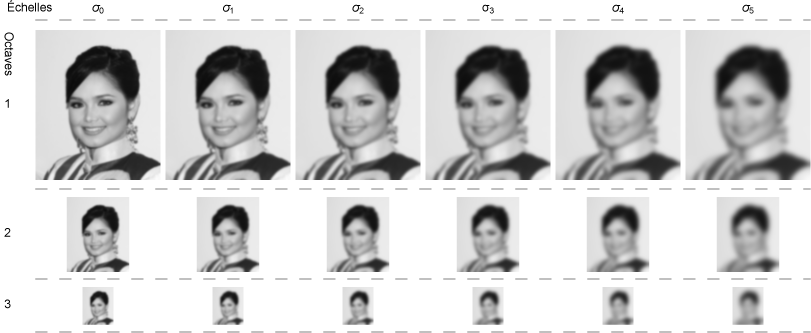
\includegraphics[width=.8\textwidth]{SIFT-scale.png}
			\caption{\label{fig:sift-scale}Espace de travail pour la détection des features avec l'algorithme SIFT. Illustration issue de \cite{frwiki:177813849}.}
		\end{figure}
		La figure \ref{fig:sift-scale} donne une illustration de cet espace de travail. Chacune des lignes correspond à une octave. La variation de taille de l'image et l'importance du flou gaussien déterminent la taille du feature en négligeant les détails qui sont de taille inférieure à $\sigma_i$.
		\\Pour chaque octave, la différence de chaque images successives est calculée pour former les différences de gaussiennes (DoG : Differences of Gaussian). La DoG issue d'images ayant des flous gaussiens $\sigma_i$ et $\sigma_{i+1}$ contient alors uniquement les détails de l'image originale dont l'échelle varie entre $\sigma_i$ et $\sigma_{i+1}$.
		\begin{figure}\centering
			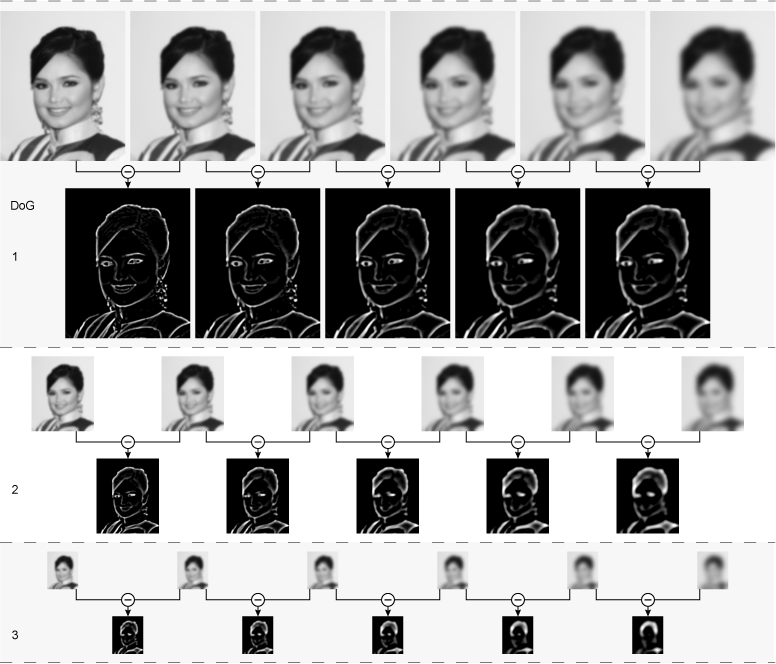
\includegraphics[width=.8\textwidth]{SIFT-DoG.png}
			\caption{\label{fig:sift-dog}Différences des gaussiennes. Illustration issue de \cite{frwiki:177813849}.}
		\end{figure}
		La figure \ref{fig:sift-dog} donne une illustration des DoG obtenues à partir des images de la figure \ref{fig:sift-scale}.
		\\Enfin, la dernière étape consiste à trouver les points d'intérêt de l'image grâce aux DoG obtenues précédemment. Il s'agit en fait d'une recherche d'extrema locaux dans l'espace des échelles. Afin de permettre cela, les DoG obtenues successivement sont placées en couche et les pixels qui ont une intensité plus petite ou plus grande que ses 26 voisins sont considérés comme des points d'intérêt.
		\begin{figure}\centering
			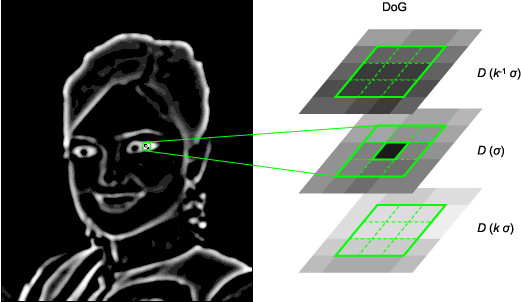
\includegraphics[width=.6\textwidth]{SIFT-PoI.png}
			\caption{\label{fig:sift-poi}Recherche des points d'intérêt. Illustration issue de \cite{frwiki:177813849}.}
		\end{figure}
		La figure \ref{fig:sift-poi} illustre la recherche d'un point d'intérêt. A l'issue de cette recherche, de trop nombreux points sont sélectionnés, une étape supplémentaire de tri est réalisé par l'intermédiaire de masques et seuillages par hystéresys.
		\paragraph{Algorithme SIFT : description des features -}
		Les features sont centrés sur les points d'intérêt et ont une taille caractéristique propre au flou gaussien en question. Une fois détectés, il est nécessaire de les décrire mathématiquement pour pouvoir les comparer. Pour accomplir cette tâche, une assignation de l'orientation et un descripteur sont calculés automatiquement de la manière présentée ci-dessous.
		\\Le calcul de l'orientation se fait à partir du calcul du gradient de l'image dans le voisinage du centre d'intérêt (convolution de l'image avec un filtre de Sobel). L'ensemble des orientations obtenues est interposée sur un histogramme à 36 valeurs (pas d'orientation de \SI{10}{\degres}) et l'orientation choisie correspond au pic dans cet histogramme, lissé auparavant. Si l'histogramme présente plusieurs pics alors le descripteur est copié et plusieurs orientations sont données pour un même point d'intérêt. La contribution de chaque pixel est proportionnelle à l'amplitude de son gradient mais aussi à la proximité avec le point d'intérêt.
		\\Vient désormais le calcul du descripteur qui est illustré sur la figure \ref{fig:sift-descr}. On considère dans un premier temps un fenêtre carrée de taille $12\sigma \times 12\sigma$ pixels centrée autour du point d'intérêt et proportionnelle à son niveau de flou de détection $\sigma$. Cette fenêtre est découpée en 16 petites fenêtres de taille $3\sigma \times 3\sigma$ pixels. Pour chaque petite fenêtre, un histogramme de l'orientation du gradient est réalisé comme précédemment sur 8 valeurs, à la différence que maintenant l'orientation du point d'intérêt est soustrait. Pour un point d'intérêt on obtient donc 16 histogrammes de 8 valeurs. Ces histogrammes sont concaténés de manière à ne former qu'un seul vecteur de 128 valeurs. Afin de rendre le descripteur invariant au changement de contraste le vecteur est normalisé. Toutes les valeurs supérieures à \num{0.2} sont remplacées par \num{0.2} de manière à rendre le descripteur insensible aux changement de luminosité également. Enfin, une dernière normalisation vient généré le descripteur du point d'intérêt analysé.
		\begin{figure}\centering
			\begin{subfigure}[c]{.45\linewidth}
				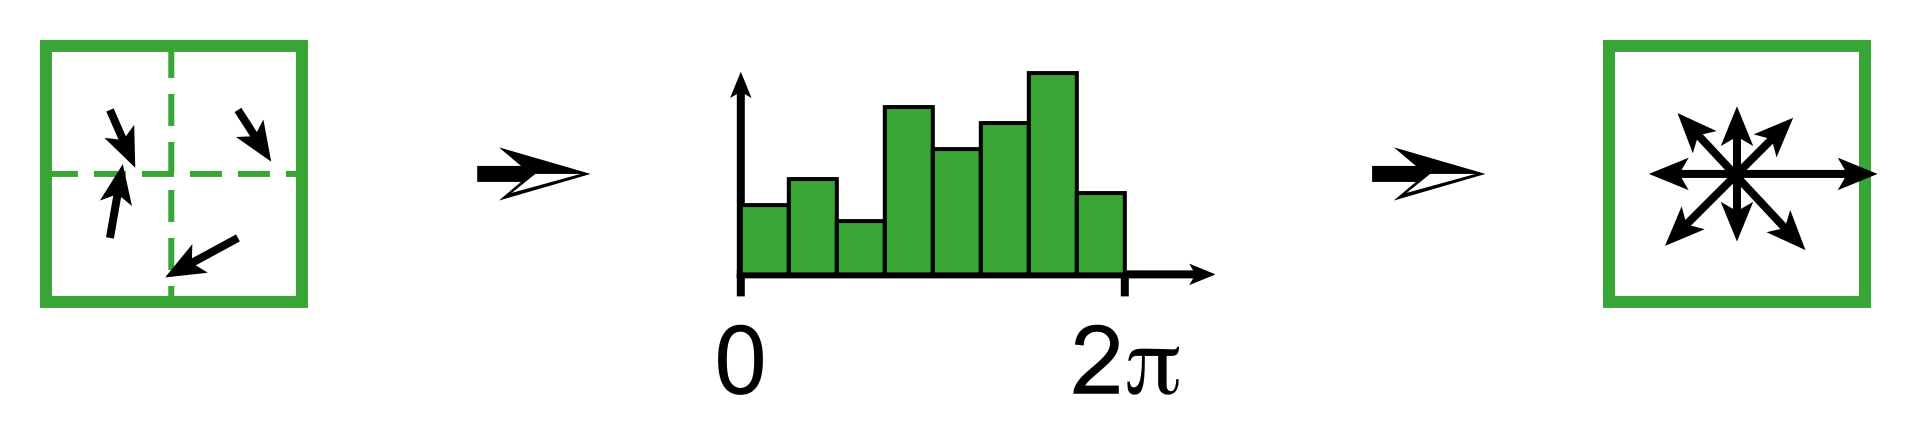
\includegraphics[width=\linewidth]{SIFT-descr02.png}
				\caption{}
			\end{subfigure}
		\begin{subfigure}[c]{.3\linewidth}
			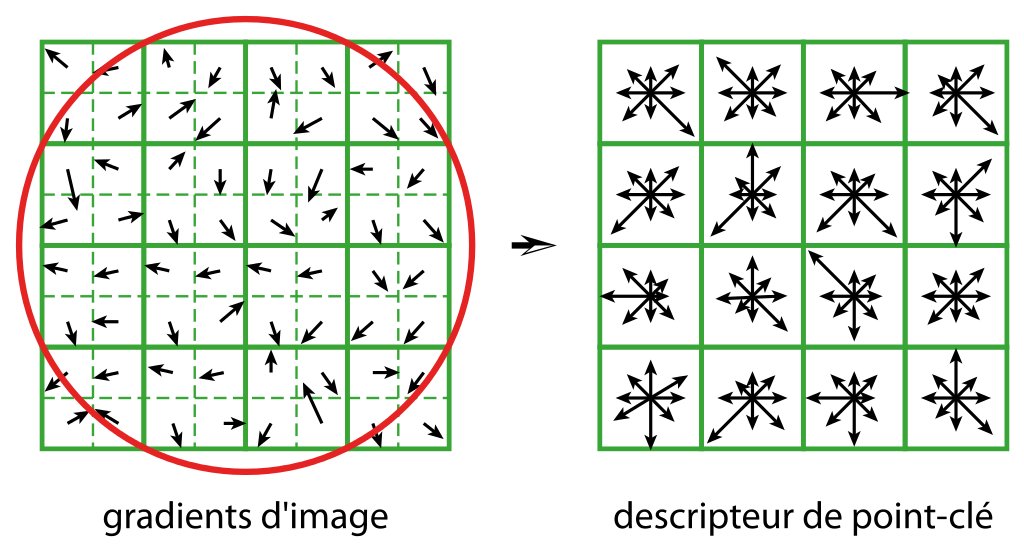
\includegraphics[width=\linewidth]{SIFT-descr01.png}
			\caption{}
		\end{subfigure}
			\caption{\label{fig:sift-descr}Méthode de calcul des descripteurs avec la méthode SIFT. Illustration issue de \cite{frwiki:177813849}.}
		\end{figure}
		\paragraph{Classification des images : machine learning -}
		Après avoir déterminé une liste de descripteurs pour l'image, il faut maintenant savoir les utiliser et les analyser grâce à un classifieur entraîné sur des images déjà classées manuellement. Il existe plusieurs moyens de classifier les images, entre autres : régression logistique, SVM (Support Vector Machine), k-plus proches voisins, forêt d'arbres aléatoires ou encore réseau de neurones. Le principe reste relativement le même pour chacune de ces méthodes : des relations plus ou moins complexes sont pondérées dans la phase d'apprentissage. Lorsque l'on souhaite faire une prédiction, ces relations pondérées sont utilisées pour déterminer la meilleure probabilité du résultat.
		\subsection*{Apprentissage automatique avec le Deep Learning}
		Les réseaux de neurones convolutifs sont très largement utilisés dans le domaine de la vision des machines. En effet, ces derniers permettent, lorsqu'ils présentent une solution de perceptrons multi-couches, d'établir des relations très complexes mais surtout de retrouver automatiquement les features utiles à la classification lors de la phase d'apprentissage. Cette solution est cependant plus lourde à mettre en \oe{}uvre puisqu'elle nécessite généralement un très long entraînement avec de nombreuses images. On peut cependant envisager de générer une multitude d'images simulées avec le logiciel Blender afin d'entraîner le réseau de neurones.

	
\end{document}
